\documentclass{article}

\usepackage{graphicx}
\usepackage{float}
\usepackage{array}

\begin{document}

  \begin{titlepage}
    \centering
    \vspace*{2cm}
    
    \Huge
    \textbf{Simulador de Polarización en Redes}
    
    \vspace{1.5cm}
    
    \Large
    Jhorman Gomez{\textsuperscript{1}}, Ivan Ausecha{\textsuperscript{2}}, James Calero{\textsuperscript{3}}, Daniel Rojas{\textsubscript{4}}
    
    \vspace{0.5cm}
    
    \large
    2326867{\textsuperscript{1}}, -{\textsuperscript{2}}, -{\textsuperscript{3}}, -{\textsuperscript{4}}
    
    \vspace{0.5cm}
    
    \Large
    Universidad del Valle
    
    \vspace{0.5cm}
    
    \large
    Facultad de Ingeniería
    
    \vspace{0.5cm}
    
    \large
    Escuela de Ingeniería de Sistemas y Computación
    
    \vspace{0.5cm}
    
    \large
    Santiago de Cali, Octubre de 2024
    
  \end{titlepage}

  \section{¿Son Nuestras Funciones Funcionalmente Puras?}

  \begin{table}[H]
    \centering
    \begin{tabular}{|c|c|p{5cm}|}
    \hline
    \textbf{Función} & \textbf{Funcional} & \textbf{¿Por qué no?} \\ \hline
    min\_p & Si & - \\ \hline
    rhoCMT\_Gen & Si & - \\ \hline
    normalizar & Si & - \\ \hline
    rho & Si & - \\ \hline
    confBiasUpdate & Si & - \\ \hline
    simulate & Si & - \\ \hline
    rhoPar & No & A pesar de que no hay efectos secundarios por el uso de paralelismo, la función no es funcionalmente pura por el no determinismo en el orden de realización de las operaciones dentro de esta. \\ \hline
    confBiasUpdatePar & No & A pesar de que no hay efectos secundarios por el uso de paralelismo, la función no es funcionalmente pura por el no determinismo en el orden de realización de las operaciones dentro de esta. \\ \hline
    \end{tabular}
  \end{table}

  \section{Técnicas y Estructuras de Datos Utilizadas}
    
    \subsection{min\_p}
    La función \textbf{min\_p} hace uso de:

    \begin{itemize}
      \item \textbf{Recursión:} genera un proceso de recursión lineal mediante el cual por cada iteración se aproxima más al punto mínimo de la función recibida.
      \item \textbf{Funciones de Alto Orden:} recibe una función como parámetro.
      \item \textbf{Colecciones:} genera un rango de valores a partir del min y max recibidos, a este rango se le aplica un map y al resultado del map se le aplica el método minBy, ambos métodos pertenecientes a colecciones.
    \end{itemize}

    \subsection{rhoCMT\_Gen}
    La función \textbf{rhoCMT\_Gen} hace uso de:

    \begin{itemize}
      \item \textbf{Funciones de Alto Orden:} hace uso de funciones anónimas y retorna esta misma como resultado.
      \item \textbf{Colecciones:} hace uso del método zip para generar una colección de tuplas (Frecuency, DistributionValue) sobre la cual se define la función sum.
    \end{itemize}

    \subsection{normalizar}
    La función \textbf{normalizar} hace uso de:

    \begin{itemize}
      \item \textbf{Funciones de Alto Orden:} hace uso de funciones anónimas y retorna esta misma como resultado.
      \item \textbf{Colecciones:} hace uso de vectores y en especial el método fill para generar una colección con la mayor polarización posible para una frecuencia de longitud k.
    \end{itemize}

    \subsection{rho}
    La función \textbf{rho} hace uso de:

    \begin{itemize}
      \item \textbf{Funciones de Alto Orden:} hace uso de funciones anónimas y retorna esta misma como resultado.
      \item \textbf{Colecciones:} hace uso de colecciones y métodos característicos de estas para generar los intervalos sobre los cuales se van a clasificar los agentes y a su vez estos se clasifican haciendo uso de métodos como map y groupBy.
      \item \textbf{Iteradores:} hace uso de métodos que requieren de iteradores como ZipWithIndex y indexWhere.
      \item \textbf{Reconocimiento de Patrones:} hace uso de reconocimiento de patrones para el reconocimiento de los elementos que hacen parte de las colecciones utilizadas, esto con el fin de poder hacer transformaciones sobre dichas colecciones y en últimas clasificar los agentes y obtener la frecuencia final a partir de las opiniones de estos.
    \end{itemize}

    \subsection{confBiasUpdate}
    La función \textbf{confBiasUpdate} hace uso de:

    \begin{itemize}
      \item \textbf{Funciones de Alto Orden:} recibe funciones como parámetro, en específico la función swg que corresponderia a la matriz de influencia.
      \item \textbf{Colecciones:} recibe una colección y en base a esta mediante el uso de map, se define la función sum sobre la que se va a realizar el respectivo update a las creencias de los agentes haciendo uso de un rango y mapeando dicha función para cada valor del rango.
    \end{itemize}

    \subsection{simulate}
    La función \textbf{simulate} hace uso de:

    \begin{itemize}
      \item \textbf{Funciones de Alto Orden:} recibe funciones como parámetro, en específico las funciones correspondientes a la matriz de influencia (swg) y la función sobre la cual se van a actualizar las creencias de los agentes (fg).
      \item \textbf{Colecciones:} recibe una colección la cual se actualiza en base a fg y mediante estas actualizaciones se va creando una secuencia indexada donde cada elemento es la creencia de los agentes en el tiempo t empezando desde t=0.
      \item \textbf{Recursión:} genera un proceso de recursión lineal sobre el cual se actualiza t-1 veces la creencia recibida (sb).
    \end{itemize}

  \section{Informe de Corrección}

    \subsection{min\_p}

    \subsection{rhoCMT\_Gen}

    \subsection{rho}

    \subsection{confBiasUpdate}

    \subsection{simulate}

  \section{Técnicas de Paralelización y Análisis de Impacto}

    \subsection{Tipos de Paralelización Usados}
    Para las funciones \textbf{rhoPar} y \textbf{confBiasUpdatePar} se utilizó solamente paralelismo de datos. A continuación  las razones:

    \begin{itemize}
      \item \textbf{rhoPar:} no hicimos uso de paralelismo de tareas porque abstracciones como \textbf{parallel} son solo útiles cuando se realizan procesos recursivos, además, la abstracción \textbf{task} realmente no tiene cabida dentro de nuestro algoritmo debido a que no es posible por ejemplo ir clasificando las creencias de los agentes antes de que todos los intervalos estén definidos.
      \item \textbf{confBiasUpdatePar:} se intentó introducir una versión paralelizada mediante paralelismo de tareas pero a la hora de realizar pruebas se llega al error stackOverFlow debido a la cantidad de memoria requerida por el programa. La versión paralelizada mediante paralelismo de tareas actual arroja resultados positivos donde se ve una aceleración en la ejecución del programa, por lo tanto, realmente no importó el detalle anteriormente mencionado.
    \end{itemize}

    A continuación el error obtenido para la versión por paralelismo de tareas en confBiasUpdate.

    \begin{figure}[H]
      \centering
      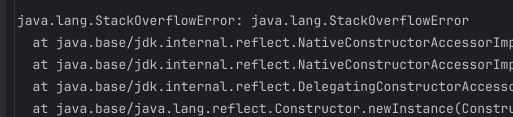
\includegraphics[width=0.8\textwidth]{images/stackOverFlow.jpg}
    \end{figure}

    \subsection{Impacto}

  \section{Pruebas y Resultados}

  \section{Conclusiones}

\end{document}